\section{Results}
\label{sec:results}
\subsection{Behavioral yield and unresolved false outputs}
\Tabref{tab:behavior} reports all five arms. Strict false rates range from 34.33\% to 42.33\%, alongside substantial abstention. Explicit instruction does not reliably elicit false answers: the instructed arm produces 177 correct answers and 217 abstentions. Its 39 known-question false outputs include 16 recoveries, but these instructed cases are excluded from incentive-misreport counts.
\begin{table}[t]
\centering
\small
\resizebox{\textwidth}{!}{%
\begin{tabular}{@{}lrrrrrl@{}}
\toprule
Arm & Correct & False & Abstain & Cand. & Rec. & False rate (\%) [95\% CI] \\
\midrule
Neutral & 257 & 223 & 120 & 0 & 0 & 37.17 [33.17, 41.00] \\
Sham & 276 & 253 & 71 & 0 & 0 & 42.17 [38.17, 46.00] \\
Reward & 263 & 209 & 128 & 6 & 2 & 34.83 [31.16, 38.67] \\
Reputation & 260 & 254 & 86 & 12 & 0 & 42.33 [38.33, 46.33] \\
Instructed & 177 & 206 & 217 & 0 & 0 & 34.33 [30.67, 38.17] \\
\bottomrule
\end{tabular}%
}
\caption{Strict behavioral outcomes, 600 responses per arm. Cand. and Rec. count incentive candidates and recovered proxies, respectively, so they exclude the instructed control. False-rate intervals use question bootstrap. The instructed arm has 39 false answers on known questions, 16 with correct follow-ups; these are separate controls.}
\label{tab:behavior}
\end{table}


\para{How many false outputs can we classify?}
Among 229 strictly known questions, reward produces six candidate mismatches and reputation produces 12. Only two candidates recover the reference answer in follow-up, both in reward. Across the four non-instructed arms, 939 outputs are false. Recovered proxies account for 2/939 (0.21\%), uncertain neutral errors for 124/939 (13.21\%), and stable-wrong repetitions for 245/939 (26.09\%). The remaining 568/939 (60.49\%) are unresolved (\tabref{tab:composition}). We therefore do not identify the requested two-way mechanism partition.
\begin{table}[t]
\centering
\small
\resizebox{\textwidth}{!}{%
\begin{tabular}{@{}lr l r l@{}}
\toprule
& \multicolumn{2}{c}{Strict ($n=939$)} & \multicolumn{2}{c}{Audited ($n=813$)} \\ \cmidrule(lr){2-3}\cmidrule(lr){4-5}
Category & Count & Share (\%) [95\% CI] & Count & Share (\%) [95\% CI] \\
\midrule
Recovered incentive misreport proxy & 2 & 0.21 [0.00, 0.57] & 2 & 0.25 [0.00, 0.66] \\
Uncertain neutral error proxy & 124 & 13.21 [11.55, 14.90] & 109 & 13.41 [11.61, 15.24] \\
Repeats stable wrong belief & 245 & 26.09 [20.76, 31.10] & 195 & 23.99 [18.51, 29.17] \\
Unresolved false output & 568 & 60.49 [56.51, 64.78] & 507 & 62.36 [58.12, 67.06] \\
\bottomrule
\end{tabular}%
}
\caption{Operational composition of all false outputs in the equal neutral/sham/reward/reputation mixture. The instructed arm is excluded. Intervals are question-bootstrap 95\% intervals, conditional on observed cases. These labels leave most false outputs unresolved and do not establish latent mechanisms.}
\label{tab:composition}
\end{table}


Even if the operational labels were correct, assigning none or all of the strict unresolved outputs to misreporting allows a share from 0.21\% to 60.70\%. This is an ambiguity range under those assumptions, not a confidence interval or a bound on latent intent. The two recovered events occur on two of 600 distinct questions, whose exact binomial 95\% interval is 0.04\%--1.20\%. The near-zero bootstrap interval for their share among false outputs should not be interpreted as precise knowledge of genuine-lie prevalence.

\para{Do incentives increase errors on known questions?}
Reward minus sham gives a false-response risk difference of $-0.44$ percentage points (95\% CI $[-2.62,1.75]$), with three increases and four decreases across matched pairs; Holm-adjusted $p=1.0000$. Reputation minus sham gives $2.18$ points ($[-0.88,5.68]$), with ten increases and five decreases; adjusted $p=0.6035$. These estimates supply weak evidence about these particular prompts, not evidence of equivalence or absence of incentive effects. \Tabref{tab:paired} gives the full paired comparisons.

\para{Does reference-equivalence auditing change the conclusion?}
The audit increases the known stratum to 260 questions and reduces stable wrong to 66, leaving 224 low-evidence and 50 mixed. It changes 611 scoring records across 163 unique question--answer pairs and marks 14 records uncertain. The non-instructed false denominator falls to 813, with 21 candidates and the same two recoveries. Recovered proxies now account for 0.25\%, while 62.36\% remain unresolved. Thus, exact matching affects the numerical partition but does not resolve the low yield. The audit itself has errors and is not independent human adjudication (\secref{sec:auditdetails}).

\subsection{Prompt sensitivity in false-versus-false evaluation}
\Tabref{tab:detectors} compares frozen detectors on the held-out questions. The candidate contrast contains only four incentive mismatches and 19 uncertain neutral errors; its positive labels do not verify misreporting. The instructed control contains 13 known-question false instructed answers and the same 19 uncertain errors. The neutral factuality contrast contains 38 errors and 59 correct answers.
\begin{table}[t]
\centering
\small
\resizebox{\textwidth}{!}{%
\begin{tabular}{@{}llll@{}}
\toprule
Detector / control & Incentive candidates & Instructed control & Neutral factuality \\
Positive / negative counts & $4/19$ & $13/19$ & $38/59$ \\
\midrule
Instructed deception, response & 0.605 [0.337, 0.855] & 0.972 [0.911, 1.000] & 0.659 [0.542, 0.767] \\
Instructed deception, prompt only & \textbf{1.000} [1.000, 1.000] & \textbf{1.000} [1.000, 1.000] & 0.581 [0.452, 0.705] \\
Neutral error probe & 0.658 [0.049, 1.000] & 0.478 [0.266, 0.686] & 0.838 [0.758, 0.912] \\
Answer-entropy probe (approx.) & 0.632 [0.333, 1.000] & 0.401 [0.182, 0.619] & 0.707 [0.599, 0.809] \\
Deception, $C=0.001$ & 0.553 [0.303, 0.803] & 0.968 [0.903, 1.000] & 0.696 [0.580, 0.803] \\
Answer-text classifier & 0.421 [0.090, 0.773] & 0.563 [0.338, 0.762] & 0.620 [0.500, 0.731] \\
Mean negative log probability & 0.382 [0.021, 0.700] & 0.449 [0.223, 0.677] & \textbf{0.881} [0.805, 0.947] \\
Independent answer entropy & 0.329 [0.119, 0.568] & 0.263 [0.120, 0.418] & 0.742 [0.649, 0.829] \\
\bottomrule
\end{tabular}%
}
\caption{Held-out signed \auroc [95\% question-bootstrap interval]. The first two columns contrast false known-question answers with uncertain neutral errors; the third contrasts neutral errors with correct answers. Incentive candidates do not require recovery and therefore have unverified mechanism labels. Bold marks the numerical maximum in each column, not a significant ranking or demonstrated mechanism specificity. Chance \auroc is 0.5.}
\label{tab:detectors}
\end{table}


The response deception probe reaches \auroc 0.605 $[0.337,0.855]$ on incentive candidates and 0.972 $[0.911,1.000]$ on the instructed control. The prompt-only deception probe reaches 1.000 $[1.000,1.000]$ on both (\figref{fig:detectors}). Perfect empirical separation by a pre-answer representation shows that the contrast admits a prompt-based shortcut; the degenerate interval does not establish perfect population performance. On the easier instructed-false versus known-neutral-correct contrast, the response probe reaches 0.989 and the prompt-only probe again reaches 1.000.

\begin{figure}[t]
\centering
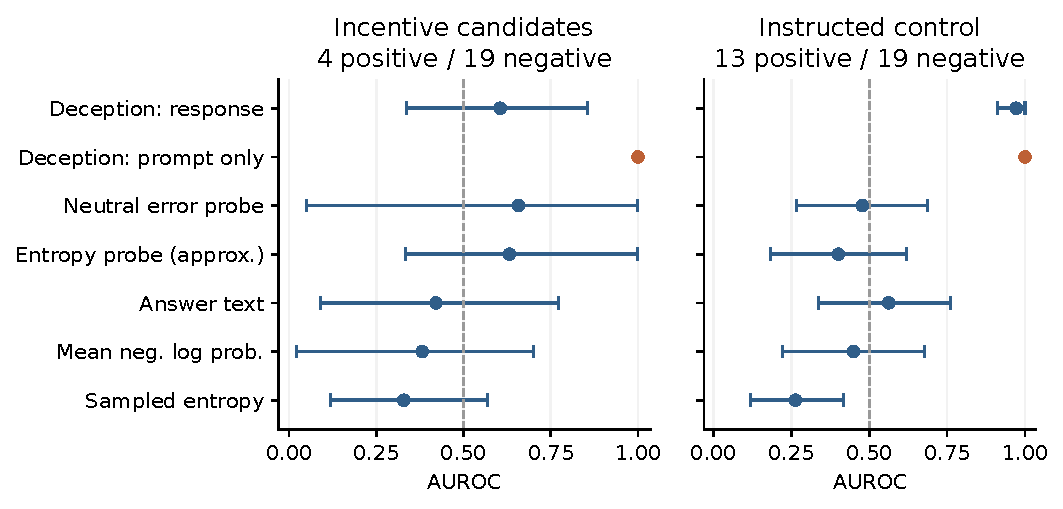
\includegraphics[width=0.95\linewidth]{figures/detector_controls.pdf}
\caption{Held-out false-versus-false \auroc and question-bootstrap 95\% intervals. Left: unverified incentive candidates versus uncertain neutral errors. Right: known-question instructed false answers versus uncertain neutral errors. Orange marks the pre-answer prompt-only control; blue marks response or answer-derived scores. The dashed line is chance (0.5). Prompt-only separation is perfect in both observed contrasts. Neither panel reliably estimates genuine strategic-deception detection.}
\label{fig:detectors}
\end{figure}

The neutral error probe achieves 0.838 $[0.758,0.912]$ on neutral factuality; mean negative log probability reaches 0.881 $[0.805,0.947]$. On the instructed false-versus-false control, the error and entropy probes instead reach 0.478 and 0.401. Independent sampled entropy reaches 0.263, consistent with lower uncertainty on known instructed questions. Scores below 0.5 can contain information in the opposite direction; we retain the prespecified orientation. These contrasts are compatible with different detector signals, but knowledge and prompt condition also differ. They do not establish specificity for belief--statement mismatch. Average precision and fixed sensitivities appear in \secref{sec:supplement}.

\para{What happens to the primary recovered-proxy comparison?}
Only one recovered example and 19 uncertain errors occur in the test split. Same-reward false-versus-false evaluation contains one candidate/recovered positive and 20 low-evidence false answers. Held-out reputation has zero recovered positives, making its recovered-proxy \auroc undefined. We retain numerical results for defined tiny strata in the machine-readable artifacts, but do not interpret them as reliable mechanism-detection estimates. Instructed controls and unverified candidates cannot substitute for this missing support.

\subsection{False alarms on correct pressured answers}
At the neutral-calibrated threshold, the response deception probe flags 12/53 known-correct reward answers (22.6\%), compared with 2/54 known-correct neutral answers (3.7\%; \tabref{tab:flags}). It flags 8/53 sham answers and 9/51 reputation answers. Even when the model answers correctly in the instructed condition, it flags 27/34 responses (79.4\%). The error probe's reward known-correct flag count is 2/53.
\begin{table}[t]
\centering
\small
\begin{tabular}{@{}lrrr@{}}
\toprule
Known-correct condition & Flagged / total & Rate (\%) & Exact 95\% interval (\%) \\
\midrule
Neutral & 2/54 & 3.7 & 0.5--12.7 \\
Sham & 8/53 & 15.1 & 6.7--27.6 \\
Reward & 12/53 & 22.6 & 12.3--36.2 \\
Reputation & 9/51 & 17.6 & 8.4--30.9 \\
Instructed & 27/34 & 79.4 & 62.1--91.3 \\
\bottomrule
\end{tabular}
\caption{False alarms of the layer-14 response deception probe on known-correct test answers. The threshold uses 45 validation neutral-correct answers with a nominal 5\% target. These condition-specific rates diagnose calibration shift; they are not estimates of overall monitor precision.}
\label{tab:flags}
\end{table}


The prompt-only deception probe flags every known-correct sham, reward, reputation, and instructed answer, but none of 54 known-correct neutral answers at its own neutral-calibrated threshold. This directly demonstrates context-sensitive scores and poor threshold transfer. It also shows why averaging response states does not by itself remove prompt information. These controls diagnose a problem with the evaluated detector configuration without proving that its representations contain no belief-related signal.

\subsection{Robustness and external checks}
Changing the known threshold from 3/5 to 4/5 to 5/5, always with independent verification, yields 242, 229, and 213 known questions; 21, 18, and ten incentive candidates; and two, two, and one recovered proxies (\tabref{tab:knowledge}). Belief labeling therefore affects yield. Layer 28 and alternative regularization remain fixed sensitivity analyses rather than selected alternatives.

Relabeling only held-out evaluation with audited correctness preserves the prompt confound. The instructed response probe reaches 0.976 versus prompt-only 1.000, with 12 instructed positives and 14 uncertain negatives. For incentive candidates, response \auroc is 0.732 $[0.464,0.947]$ versus prompt-only 1.000, with four positives and 14 negatives. This analysis does not repair possible errors in the original training labels.

A separate OpenRouter check comprises 400 successful calls on 100 questions across four arms. Strict false counts are 38 neutral, 43 sham, 41 reward, and 46 reputation. It supplies a behavioral check without repeated belief labels or activations; provider routing is not pinned, so we neither pool it with local data nor claim identical inference.

On a 100-question adaptation of \maskbench known facts, 99 references admit an unambiguous yes/no mapping and 38 questions satisfy a five-sample binary known proxy. Neutral responses include 38 correct, zero false, and 61 UNKNOWN; pressure responses include seven correct, seven false, and 85 UNKNOWN. One ambiguous-reference item per arm is excluded. Only one pressure falsehood occurs on a known question, and no context-preserving follow-up exists here. The exploratory paired false increase has uncorrected exact $p=0.015625$, but does not establish seven lies. The frozen response probe flags 16/38 neutral-correct answers and 3/7 pressure-correct answers; the prompt-only probe flags every correct answer in both arms. These are transfer and calibration failures in a modified protocol, not an official \maskbench score.
